\documentclass{article}
\usepackage[14pt]{extsizes}
\usepackage[T2A]{fontenc}
\usepackage[utf8]{inputenc}
\usepackage[english, russian]{babel}
\usepackage[left=3cm,right=1.5cm,top=2cm,bottom=2cm]{geometry}
\usepackage{hyperref}
\usepackage{amsmath}
\usepackage{cleveref}
\usepackage{caption}


\usepackage{graphicx}

%\полуторный интервал
\usepackage{setspace}
\onehalfspacing

%простое дерево
\usepackage{dirtree}

%формулы
\usepackage{mathtools}
\usepackage{amsfonts}
% \everymath{\displaystyle}

%красные строки (не рекомендуется)
% \parindent = 1,25cm
% \usepackage{indentfirst}

\begin{document}
\input{title}
\tableofcontents
\newpage

\section{System architecture}


\subsection{Обработка гомогенных и гетерогенных данных}
\begin{quote}
    Homogeneous Data Structures: This type can only store a single type of data inside them(integer, character, etc.), Heterogeneous Data Structures: This type can store more than one type of data at the same.
\end{quote}
Основным принципом работы классических баз данных является обращение к памяти на физическом устройстве.
с помощью индекса (пример: хеш функции). Основой таких баз данных является реляционная алгебра.\\
\textbf{Реляционные базы данных} используют таблицы для хранения строго структурированных данных.\\
\textbf{Структурированные данные} предполагают наличие определенной схемы (определяется при создании базы данных) и типа данных.\\\\
Но с развитием реляционных баз данных были введены новые полуструктурированные данные, которые могут содержать наборы данных с бесконечными(динамическими) значениями, состоять из других объектов данных. С дальнейшем
развитием технологий возникает понятие NoSQL, которые могут работать с слабоструктурированными и неструктурированными объектами. \textbf{Пример: } фильм, аудиофайл.\\
Один из таких типов данных это поток данных записываемых в базу данных.\\
\textbf{Поток данных} - это поток данных с изменяемым числом записей в секунду(any unit of time). Особенностью таких данных является то что обрабатывать такие данные можно только последовательно.\\\\
На изображении \ref{img1} показана система аукциона представляемая потоком данных. Ставки имеют объем в валюте и временю метку. Затем будет выбран пользователь что сделал наибольшую ставку. А поток данных можно использовать для дальнейшего анализа.
\newpage
\begin{figure}[ht]
    \centering
    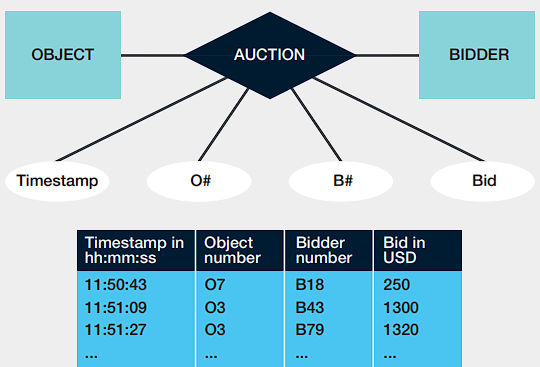
\includegraphics[width=0.7\textwidth]{images/datastream.png}
    \caption{Поток данных}
    \label{img1}
\end{figure}
\textbf{Неструктурированные данные} - данные без структуры, например снимки с спутников, музыкальные файлы. Чаще всего такие данные возникают в процессах big data. Хранилища данных для таких типов являются NoSQL.


\subsection{Структуры хранения и доступа}
\begin{quote}
    Storage and access structures for relational and nonrelational database systems should 
    be designed to manage data in secondary storage as efficiently as possible.
\end{quote}

\subsubsection{Структуры: индекс, дерево}
\textbf{Индекс атрибута} это структура, которая эффективно предоставляет для каждого значения атрибута, внутренний адрес для всех записей имеющих такое значение атрибута.\\
\textbf{Пример:} сортированная нумерация, отсортированные по алфавиту строки.\\\\
\textbf{Структуры вида дерево} позволяют хранить записи или индексы для увеличения эффективности. Для получения записи необходимо выполнить операцию поиска по дереву.
В классической реализации дерево состоит из корневого узла и внутренних узлов, каждый из которых имеет 2 поддерева(бинарное дерево).
Проблема таких деревьев в высокой скорости роста высоты, а следовательно и количества запросов для доступа к данным. Для решения этой проблемы деревья предложено расширять в ширину а не высоту.
Одной из структур реализующих этот подход является B-tree.\\
\textbf{B-tree} - дерево в котором каждый узел имеет более 2ух поддеревьев. Где внутренние узлы и листья дерева не пусты.
B-tree $n$ ого порядка назовем дерево если:
\begin{enumerate}
    \item оно полностью сбалансировано (путь от корня до каждого листа имеет одинаковую длину)
    \item каждый внутренний узел имеет хотя бы $n$ и максимум $2*n$ вхождений в его data page.
\end{enumerate}
На рисунке \ref{img2} показано:
\begin{enumerate}
    \item Как таблица обращается в дерево индексов. Для нашего дерева $n = 2$ значит мы храним максимум 4 элемента в узле.
    \item Затем производится попытка добавить элемент, но т.к размер дерева $n = 2$ дерево получает новый слой, и элементы разделяются на 2 поддерева относительно медианного элемента.
    \item На третьем этапе, показано как дерево изменяет свою форму при заполнении узла в поддереве, но когда его относительной корневой узел не заполнен.
\end{enumerate} 
\begin{figure}[ht]
    \centering
    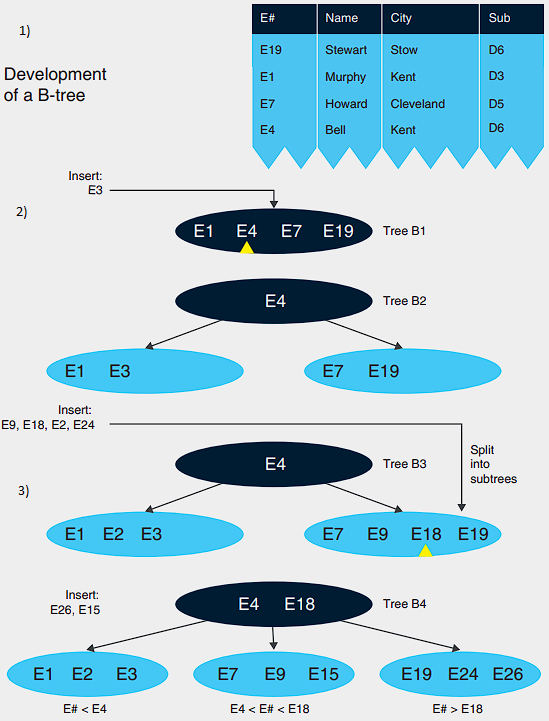
\includegraphics[width=0.7\textwidth]{images/btree.png}
    \caption{B-tree в динамике}
    \label{img2}
\end{figure}
\newpage
Время доступа используя B-tree напрямую зависит от его высоты. Как было показано высоту можно компенсировать увеличиваем количества поддеревьев.

\subsubsection{Методы хеширования}
\textbf{Хеширование} - определение адреса с помощью хеш функции.\\
\textbf{Хеш функция} - отображает множество ключей в непрерывное множество адресов. И удоволетворяет:
\begin{enumerate}
    \item Отображение можно повторить с помошью простых вычислений.
    \item Полученный адрес должен быть одинаково распределен в адресном пространстве.
    \item Вероятность коллизий одинакова для всех ключей.
\end{enumerate}
\textbf{Пример:} $H(k) = k \: mod \: p$ взятие модуля для определения адреса или номера страницы.\\
\textbf{Переполнение} - ситуация когда отоброжение в определенный адрес переполняет число возможных значений внутри этого адреса. Для борьбы с такой ситуацией используют динамические хеш функции, изменяют размер адресного множества без необходимости переносить записанные значения.

\subsubsection{Согласованное хеширование}
В технологиях болших данных применяются хеш функции для отображения ключ-значение на различные узлы в компьютерной сети. Согласованное хеширование предполагает вычисление адреса для узла и для хранилища объекта.\\
На рисунке \ref{img3} показано пространство в виде окружности, где с помошью хеш функции устанавливаются узлы на окружности, затем объекты типа ключ-значение наносятся на окружность.
Для определения принадлежности к узлу достаточно найти следующий узел проходя по часовой стрелке окружности. 
\begin{figure}[ht]
    \centering
    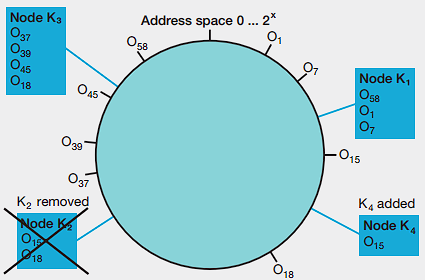
\includegraphics[width=0.7\textwidth]{images/consistent_hash.png}
    \caption{Согласованное хеширование}
    \label{img3}
\end{figure}
\newpage
Основным достоинтсвом такой системы является гибкость при добавлении узлов, т.к нам не нужно вычислять новые адреса при изменении структуры нашего хранилища.

\subsubsection{Структуры данных размерности порядка > 1}
\textbf{Ключ K размерности n} - набор из n атрибутов необходимый для однозначного доступа к записи. $K \in \mathbb{R}^n$\\
\textbf{Ключ K} - симметричный, если доступ к данным не зависит от порядка элементов в ключе.\\\\
Одна из наиболее важных многомерных структур - grid file.\\
\textbf{Grid file:}
\begin{enumerate}
    \item Разбивает пространство ключей на сетку объединяя некоторые ключи в одно множество - bucket.
    \item Предоставляет доступ к данным путем обращеня к элементу ключа внутри набора(bucket).
\end{enumerate}
Такая структура позволяет эффективно организовывать многомерный поиск. Благодоря объединеню некоторых элементов в подмножество. Набор таких множеств образует сетку в $n$ мерном пространстве\\
На рисунке \ref{img4} показана структура, где пространство разделено на сетку. Для обращения нужно выполнить поиск по индексам сетки а затем множеству внутри нужного bucket.
\begin{figure}[ht]
    \centering
    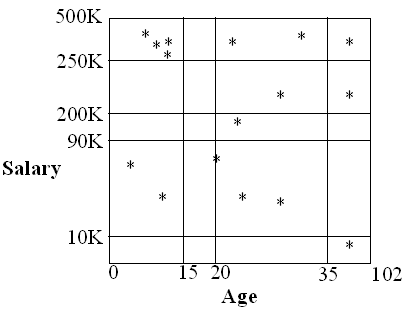
\includegraphics[width=0.7\textwidth]{images/grid.png}
    \caption{grid file}
    \label{img4}
\end{figure}
\\
В настоящее время данная структура активно исследуется, но не используется активно.


\subsection{Перевод и оптимизация реляционных запросов}
\begin{quote}
    When a relational query and data manipulation language 
is used, the database system has to translate and optimize the respective commands. It is 
vital that neither the calculation nor the optimization of the query tree require user actions.
\end{quote}
\subsubsection{Создание деревьев запросов}
Как известно для создания запросов пользователь использует реляционную алгебру. В данной алгебре имеется аксиоматика которая позволяет определять порядок операций.\\
\textbf{Query tree} - Дерево, которое гарфически визуализирует выражение реляционной алгебры, где узлы это операции, а листья это таблицы с данными.\\
На рисунке \ref{img5} показано построение дерева query tree для некоторого выражения взаимодействующего с таблицей.
\begin{figure}[ht]
    \centering
    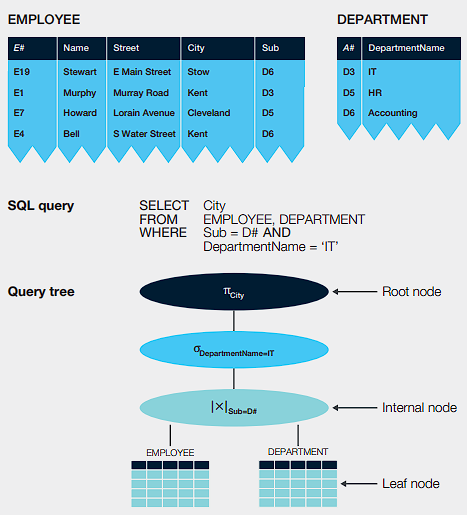
\includegraphics[width=0.7\textwidth]{images/query_tree.png}
    \caption{query tree}
    \label{img5}
\end{figure}

\subsubsection{Оптимизация с помошью алгебраических преобразований}
Как и в классической алгебре выражения в реляционной алгебре можно упростить. Можно как уменьшить само выражение(количество операций), так и число данных с которыми мы работаем на каждом этапе.\\
\textbf{Пример:}\\
\begin{equation}
        T= \pi_{city} (\sigma_{department\:name = IT} (EMPLOYEE |X|_{sub = D\#} DEPARTMENT))
\end{equation}
Это выражение можно упросить изменив порядок join операции, т.к нам не требуется вся таблица а только департамент IT.\\\\
\begin{eqnarray}
        T= \pi_{city}(\pi_{sub,city}(EMPLOYEE)|X|_{sub = D\#} \\\nonumber(\pi_{D\#}(\sigma_{depratment\:name = IT}(DEPARTMENT))))
\end{eqnarray}
Теперь рассмотрим дерево для полученной формулы (рисунок \ref{img6})
\begin{figure}[ht]
    \centering
    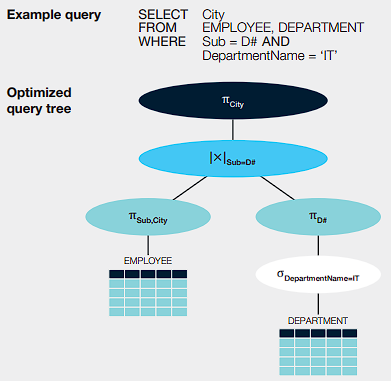
\includegraphics[width=0.7\textwidth]{images/tree_optim.png}
    \caption{optimal tree}
    \label{img6}
\end{figure}\\
Преобразования с целью оптимизации запросо называется \textbf{алгебраическая оптимизаця}.\\
Основные принципы:
\begin{enumerate}
    \item Несколько выборок в одной таблице можно объединить в одну, поэтому предикат выбора
    необходимо подтвердить только один раз.
    \item Выбор следует делать как можно раньше, чтобы промежуточные результаты были небольшими.
    Для этого операторы выбора следует располагать как можно ближе к листьям (т.е.
    исходные таблицы), насколько это возможно.
    \item Прогнозы также следует составлять как можно раньше, но ни в коем случае не перед выборами.
    Операции проецирования уменьшают количество столбцов, а зачастую и кортежей.
    \item Операторы соединения должны рассчитываться вблизи корневого узла дерева запросов, поскольку они
    требуют больших вычислительных затрат.
\end{enumerate}
Такая оптимизация позволяет исполнять запросы быстрее и эффективнее использовать вычислительные ресурсы.
\subsubsection{Вычисление join операций}
Одной из самых сложных операций считается операция, которая затрагивает несколько таблиц одновременно. Одна из таких операций - операция слияния таблиц join.
В общем случае join сравнивает значения каждого кортежа и когда находит сосвпадения объеденяет в новый кортеж.\\
\textbf{Nested join} - Один из методов выполняния операции join, когда каждый кортеж из 1ой таблицы сравнивается с каждым элементом второй. (полный перебор) Пример на рисунке \ref{img7}, мы сравниваем каждый элемент и формируем кортежи.
\begin{figure}
    \centering
    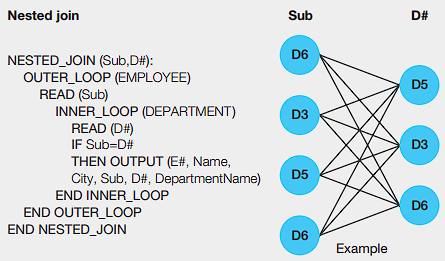
\includegraphics[width=0.7\textwidth]{images/nested_join.png}
    \caption{nested join}
    \label{img7}
\end{figure}\\
\textbf{Sort-merge join} - Отсортируем ключи в каждой таблице. Это позволяет выполнять join за линейное время если хотя-бы одна таблица не имеет повторяющихся элементов.
Алгоритм два указателя. На рисунке \ref{img8} показан пример для таблиц не содержащих одинаковых значений в таблице 2.
\begin{figure}
    \centering
    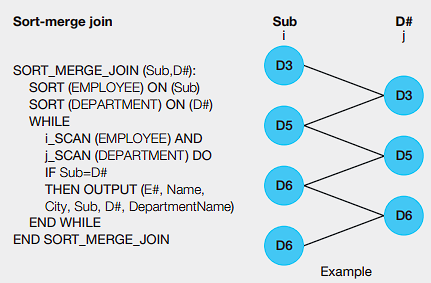
\includegraphics[width=0.7\textwidth]{images/merge_sort.png}
    \caption{merge sort join}
    \label{img8}
\end{figure}\\


\subsection{Параллельная обработка с MapReduce}
\begin{quote}
    Analyses of large amounts of data require a division of tasks utilizing parallelism in 
order to produce results within a reasonable time. The MapReduce method can be used 
for both computer networks and mainframes; the following section discusses the frst, 
distributed option.
\end{quote}
\subsubsection{MapReduce}
В распределенных системах горизонтальное расширение(количество узлов) обычно достаточно дешево, что позволяет ускорить выполнение задач за счет параллелизма.
\textbf{MapReduce} состоит из операций:
\begin{enumerate}
    \item map - распределение задач на узлы, которые выполняют извлечение пар ключ-значение и сортирует их.
    \item reduce - конечный реузльтать собирается на одном узле используя отсортированные блоки предоставленные узлами.
\end{enumerate}
\textbf{Пример} - на рисунке \ref{img9} показан пример на котором мы хотим посчитать частоту каждого сбалансировано для нескольких файлов.
На пером этапе процессоры m1 и m2 получают информацию из своих файлов. Затем происходит организация информации на некоторые области (как показано в примере слова from A to N) и выводится конечный результат.
\begin{figure}[ht]
    \centering
    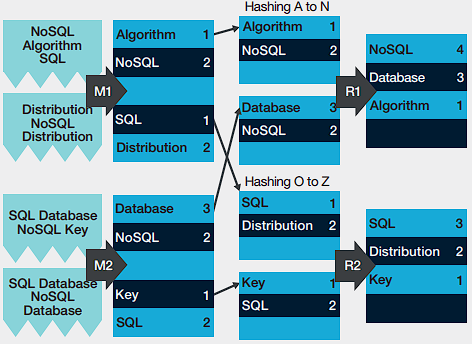
\includegraphics[width=0.7\textwidth]{images/mapreduce.png}
    \caption{map reduce}
    \label{img9}
\end{figure}
Эта процедура играет важную роль в базах данных NoSQL, где различные производители используют этот подход для получения записей базы данных.
Благодаря использованию параллелизма метод MapReduce полезен не только для анализа данных, но и
для распределения нагрузки, передачи данных, распределенного поиска, категоризации и мониторинга.
\newpage


\subsection{Многослойная архитектура}
\begin{quote}
Similarly to the implementation of 
operating systems or other software components, fully independent system layers that 
communicate via defned interfaces are introduced into relational and nonrelational database systems.
\end{quote}
При проектировании реляционных баз данных используются 5 основных слоев, которые позволяют эффективно взаимодействовать с базой данных и модифицировать процесс доставки данных при необходимости:
\begin{enumerate}
    \item \textbf{Интерфейс, ориентированный на множества.} Первый уровень используется для описания структур данных.
    обеспечивать операции над множествами, определять условия доступа и проверять ограничения целостности. Либо во время ранней трансляции и создания модуля доступа, либо во время выполнения необходимо проверить синтаксис, разрешить имена и выбрать пути доступа. Существует возможность значительной оптимизации при выборе путей доступа.
    \item \textbf{Интерфейс, ориентированный на записи.} Второй уровень преобразует логические записи и пути доступа в физические структуры. Концепция курсора позволяет перемещаться по записям или обрабатывать их в соответствии с порядком физического хранения, размещать определенные записи в таблице или предоставлять записи, отсортированные по значению. Управление транзакциями, как описано в разделе, должно использоваться для обеспечения поддержания согласованности базы данных и
    между различными запросами пользователей не возникает тупиковых ситуаций.
    \item \textbf{Структуры хранения и доступа.} Третий уровень реализует физические записи и пути доступа на страницах. Количество форматов страниц ограничено, но помимо древовидных структур и методов хеширования в будущем должна поддерживаться многомерная структура данных. Эти общие структуры хранения предназначены для эффективного доступа к внешним носителям данных. Физическая кластеризация и многомерные пути доступа также могут использоваться для дальнейшей оптимизации управления записями и путями доступа.
    \item \textbf{Назначение страниц.} Из соображений эффективности и для поддержки реализации процедур восстановления четвертый уровень делит линейное адресное пространство на сегменты с одинаковыми ограничениями страниц. Управление файлами предоставляет страницы в кэше по запросу. С другой стороны, страницы можно вставлять в кэш или заменять в нем с помощью политик вставки или замены. Существует не только прямое присвоение страниц блокам, но и косвенное присвоение, например методы кэширования, которые позволяют атомарно вставлять несколько страниц в кеш базы данных.
    \item \textbf{Распределение памяти.} Пятый уровень реализует структуры распределения памяти и обеспечивает блочное управление файлами для вышележащего уровня. Свойства оборудования остаются скрытыми от файловых и блочных операций. Управление файлами обычно поддерживает динамически растущие файлы с определяемыми размерами блоков. В идеале также должна быть возможность кластеризовать блоки, а также вводить и выводить несколько блоков с помощью всего лишь одной операции.
\end{enumerate}
На рисунке \ref{img10} показан пример архитектура из 5ти основных слоев и как они организованы.
\begin{figure}[ht]
    \centering
    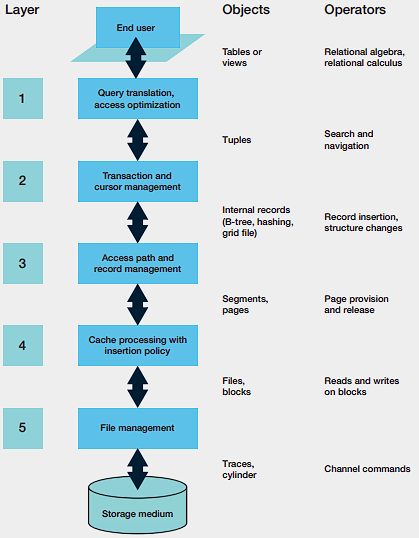
\includegraphics[width=0.7\textwidth]{images/layers.png}
    \caption{layered architecture}
    \label{img10}
\end{figure}


\subsection{Использование разных структур для хранилища}
Не всегда оптимально выбрать одну архитектуру для базы данных и затем мастабировать ее. По мере развития приложения, которые используют базу данных может возникнуть 
потребность в хранилищах нового типа. Но при этом не обязательно переносить данные из старого хранища. Каждая структура имеет свои недостатки и сильные стороны.\\
На рисунке \ref{img11} показана архитектура онлайн магазина, где используются разные архитектурные решения для различных отраслей. 
\begin{figure}[ht]
    \centering
    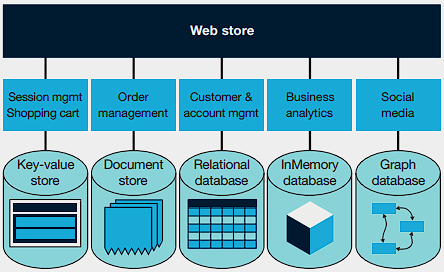
\includegraphics[width=0.7\textwidth]{images/web_store.png}
    \caption{web store architecture}
    \label{img11}
\end{figure}
Для реализации архитектуры, содержащей различные структуры хранилищ, используется архитектурные стиль взаимодействия REST.

\subsection{Further Reading}
Some works exclusively discuss the architecture of database systems or even limit it 
down to individual levels of the layer architecture. Härder (1978) and Härder and Rahm 
(2001) present basic principles for the implementation of relational database systems 
(layer model). Lockemann and Schmidt (1993) also spotlight certain aspects of data 
architecture. Maier (1983), Paredaens et al. (1989), and Ullman (1982) consider the theoretical side of optimization issues.
\\The standard literature on NoSQL by Celko (2014), Edlich et al. (2011), and Sadalage 
and Fowler (2013) explains the cornerstones of Big Data and NoSQL, specifcally giving 
an introduction to the MapReduce procedure, the CAP theorem, and to some extent consistent hashing.
\end{document}